\documentclass[main]{subfiles}

\begin{document}

\section{How concurrency is achieved: Processes and Threads}
\subsection{Disclaimer}
% Make reference to useful learning materials such as Herlihy, Sophormic Intro and lecture slides/exercises
This section introduces the concepts of parallelism and threading, which are based heavily in operating systems. However, no operating systems background is required for this course and some OS concepts necessary to understand threading are included in this section. This gives the reader more context and intuition. % Subsections diverging far from the lecture topics are marked with \textit{'Digression'}. These subsections cover questions that might come up while reading and are neither covered by the lecture, nor relevant for the exam.

% sources: Thread states in Java: https://docs.oracle.com/javase/8/docs/api/java/lang/Thread.State.html
% Thread states and diagram: https://www3.ntu.edu.sg/home/ehchua/programming/java/j5e_multithreading.html
% os basics: processes, threads: https://web.archive.org/web/20201004050736/http://pages.cs.wisc.edu/~remzi/OSTEP/cpu-intro.pdf

\subsection{Threads and Processes from the OS Perspective}
A modern computer can run hundreds of programs at the same time with only a few cores. To achieve this, the OS organizes programs into processes and threads.\\
A process is an abstraction the OS provides us for something we can informally define as a \textit{running program}. When we run a program on a computer, the OS will create a process and allocate resources such that it can execute. A process is defined by its \textit{context} or \textit{state}:
\begin{itemize}
    \item CPU register contents (including special registers like program counter and stack pointer).
    \item Memory contents in its address space.
    \item Information about I/O (like open files).
\end{itemize}
This state is stored in the process table, which maps each process id to a so-called \textit{process control block}. The process control block holds the context of the process. \\[3mm]
Processes are further divided into threads. Each process consists of at least one thread, and all threads in a process share the same address space, hence can see the same memory. This also means that threads within the same process can communicate easily using shared variables. Threads are much more light-weight than processes since they inherit much of their state from their parent process.

\subsubsection{Scheduling and Context Switches}
By introducing these OS concepts, the notion of parallelism boils down to how the OS divides the resources (CPU cores and memory) on the competing processes and threads. Imagine we have an n-core CPU. The OS can schedule n threads to execute at any time. Scheduling is done in three granularities:
\begin{itemize}
    \item \textit{Long-term scheduling}: Admits or rejects processes to the set of managed processes.
    \item \textit{Medium-term scheduling}: Decides which of the managed processes are in main memory at any given time and can swap out processes from main memory to secondary memory (usually disk).
    \item \textit{Short-term scheduling}: Concerns which threads currently loaded into memory get CPU access time.
\end{itemize}
We are concerned only with short-term scheduling in this course and whenever scheduling is mentioned, short-term scheduling is meant. The short-term scheduler, or CPU scheduler, decides which n threads get CPU access time at any given moment. We assume a \textit{pre-emptive scheduler}, which just means that the scheduler can interrupt a thread at any time and swap it out for another thread, even if the thread didn't finish executing all its instructions yet.\\
Descheduling a thread in favour of another is called a \textit{context switch}. Upon a context switch, the OS has to store the context of the descheduled thread to memory and load the context of the newly scheduled thread from memory to the CPU core the thread is going to run on. This is quite expensive and hence the OS does not want to context switch too frequently. The short-term scheduler deals with threads instead of processes since they have much less context to load from and to memory than processes.

\subsubsection{Concurrency vs Parallelism}
When two threads are now scheduled at the same time on different cores, they are executing in \textit{parallel}. However, we say that two threads are running \textit{concurrently}, when their lifetime overlaps. Two threads can run concurrently without ever being scheduled at the same time.\\
It is easy to show this on a single-core CPU. Imagine the OS only has two threads and keeps context switching between them. These threads run concurrently without ever actually executing instructions at the same time.\\
Imagine a scenario again with two threads and a single core. The OS can decide to schedule the first thread until it completes and dies. It then schedules the second thread until it completes its tasks and dies. Even though the actual execution time of the first and second thread do not overlap, we still say that they run \textit{concurrently}, because their lifetime overlaps (the second thread was \textit{runnable}, but not scheduled while the first thread was scheduled). We see that concurrency is more of a conceptual property of a program; multiple tasks/threads are order-independent and \textit{can} be run in parallel.\\
On a high level, we could say that concurrency is about \textit{dealing} with multiple things at the same time, while parallelism is about \textit{doing} these things at the same time.

% \subsection{\textit{Digression}: Why does my CPU claim 4 cores and 8 threads? Simultaneous Multi-Threading}
% On some PC's specification sheet n cores and 2n threads are listed. We also say that there are 2n logical cores. To the OS, the CPU appears to have 2n cores, meaning that it can schedule 2n threads at the same time. To understand this, we first need to understand that modern CPU's are pipelined.\\
% We imagine a simplified CPU with 5 pipeline stages: Fetching, decoding, operand fetching, computation and write-back. In each clock cycle, a new instruction is fetched and each instruction already in the pipeline moves on to the next stage, except when the operands of any instruction are not available yet (dependencies in the code). In this case, all instructions before that one in the pipeline are stalled until the operands are available.\\
% Consider the two toy programs A and B, which are compiled to the following machine code:
% \\A:
% \begin{minted}[]{gas}
% MOV $0 %eax          // A1: %eax <- 0
% ADD %eax %eax        // A2: %eax <- %eax + %eax
% \end{minted}
% B:
% \begin{minted}[]{gas}
% XOR %ebx %ebx        // B1: %ebx <- %ebx XOR %ebx
% ADD $5 %ecx          // B2: %ecx <- %ecx + 5
% MUL %ebx %ebx        // B3: %ebx = %ebx x %ebx
% \end{minted}
% We label the instructions A1, A2 and B1, B2, B3. Because of dependencies in the programs, both A and B have to stall the pipeline once and the overall execution takes 12 cycles when first fetching A1, A2, then B1, B2, B3. In practice, between A2 and B1 a context switch happens from thread A to thread B, which takes many cycles to complete, since all register values of thread A have to be loaded to memory and the context of thread B has to be loaded from memory.\\
% Now assume we have an Intel CPU supporting Intel's SMT implementation called Hyperthreading. In this case, there are two copies of all registers, one for each thread. Hence, both thread A and B have their context saved in registers at the same time. Now, the CPU can decide in each cycle whether to fetch the next instruction of thread A or thread B. Whenever a dependence occurs, the CPU can just fetch an instruction of the other thread instead of stalling the pipeline. In our toy example, this will look like this:\\
% The two advantages of SMT are that:
% \begin{enumerate}
%     \item Less context switches are required, since multiple thread contexts can be loaded into each core at the same time.
%     \item The pipeline has to stall less, since we can fetch independent instructions of another thread whenever dependencies or memory accesses occur.
% \end{enumerate}
% Most modern Intel CPU's implement SMT by providing twice the amount of registers per CPU core, such that two threads can be running concurrently without context switching. From above example, it should be clear that this approach does not give a 2x speedup. However, it is effective at decreasing so-called bubbles in the pipeline and hence maximizing resource usage.
%
% To conclude, the OS can treat such a system as having 2n cores, since it can schedule 2n OS threads at any given point in time. Note that the factor of 2 is well-chosen, but could also be any other positive integer m, as long as there are m copies of the architectural registers in each core.
%
\subsection{Java Threads}
The concept of a thread exists in multiple layers of abstraction. What we talked about so far are threads on the OS level. These are used as a means of organising running programs on the system.\\
Programs themselves can also expose threads to the programmer. In many languages, these are so-called \textit{virtual threads} or \textit{green threads} and have to be treated as an additional level of abstraction, since they are managed by the language itself and not the OS. In Java however, the thread library exposed by the language is very closely related to actual OS threads, since user created threads are 1-to-1 mapped to OS threads. Thus, we can talk about Java threads on the same abstraction level we did so far. Every executing program in Java is made up of threads. Even a normal single-threaded Java program runs on the \textit{main thread}.
We can imagine a Java thread as a sequence of [Java] instructions that are executed sequentially.

\subsubsection{Creating Java Threads}
We demonstrate three viable methods of creating Threads from within a Java program.
\begin{enumerate}
    \item Create a custom class implementing the runnable interface.
    \begin{minted}[]{java}
    public class myRunnable implements Runnable {
        public void run() {
            /* write code to be executed upon
            starting the thread here
            */
        }
    }
    \end{minted}
    Now we can instantiate this class in our code, construct a Thread instance with it and have its run method execute concurrently on another thread:
    \begin{minted}[]{java}
    myRunnable R = new myRunnable();
    Thread T = new Thread(R);
    T.start(); // starts T and executes its run() method
    \end{minted}
    We start a thread by calling start() on an object instance. Note that we can also execute the run() method of a Runnable or Thread by simply doing a function call:
    \begin{minted}[]{java}
    myRunnable R = new myRunnable();
    Thread T = new Thread(R);
    T.run(); // usually not what we want
    \end{minted}
    This executes the run method on the same thread instead of creating a new one and is usually not what we want.
    Keep in mind that this is a normal Java class and we could add other methods, fields and constructors.

    \item Extend the Java Thread class:
    \begin{minted}[]{java}
    public class myThread extends Thread {
        public void run() {
            /* write code to be executed upon
            starting the thread here
            */
        }
    }
    \end{minted}
    Note that using this method, our myThread class cannot extend another class, while using the first method this would be possible.\\
    We can now instantiate the myThread class and start the instanciation.
    \begin{minted}[]{java}
    myThread T = new myThread();
    T.start(); // starts T and executes its run() method
    \end{minted}

    \item The most compact method is to create the code that is run by the thread anonymously and inline:
    \begin{minted}[]{java}
    Thread T = new Thread() {
        public void run() {
            /* write code to be executed upon
            starting the thread here
            */
        }
    };
    T.start();
    \end{minted}
\end{enumerate}

\subsubsection{Daemon vs Non-Daemon Threads}
Java differentiates daemon threads that are responsible for background tasks like memory management (for example the garbage collector is a daemon thread) and non-daemon threads, which execute the program itself. The main thread is non-daemon and so are all user-created threads by deafult.\\
A Java program only terminates once all non-daemon threads die. This means in particular that non-daemon threads can continue to run, even when the main() method returned.\\
Manually created threads are non-daemon by default, but can be made daemon threads using the setDaemon( boolean ) method. This can only be done before the thread is started. In this course however, we will exclusively work with non-daemon threads.

\subsubsection{Thread states}
If we want to be able to talk about the effects of different thread operations, we need some notion of \textit{thread states}. In short, a Java thread typically goes through the following states:
\begin{itemize}
    \item \textit{New}: Once the \texttt{Thread} object is created, the thread enters the new state. At this point, the thread is just an object in the heap and no resources have been allocated for it.
    \item \textit{Runnable}: Once we call \texttt{start()} on the new thread object, the system allocates resources to enable its execution and the thread becomes eligible for being scheduled.
    \item \textit{Running}: When the thread is actually scheduled to run.
    \item \textit{Not runnable}: We use this as an umbrella state for multiple states that cause the thread to not be runnable. The thread enters this state when one of the following events occur:
        \begin{enumerate}
            \item The sleep() method is called to suspend the thread for a specified amount of time to yield control to the other threads.
            \item The wait() method is called to wait for a specific condition to be satisfied.
            \item The thread is blocked and waiting for an I/O operation to be completed. Attempting to acquire a lock and calling join() will also cause a thread to be blocked, but these two topics will be covered later on.
        \end{enumerate}
    These methods and terms will be covered in the next chapter. At this point we just note that even though our Java threads are scheduled by the OS, we still have \textit{some} control over them from the language itself.
    \item \textit{Terminated}: A thread transitions to terminated state when the run() method terminates and exits.
\end{itemize}
\begin{figure}[H]
    \centering
    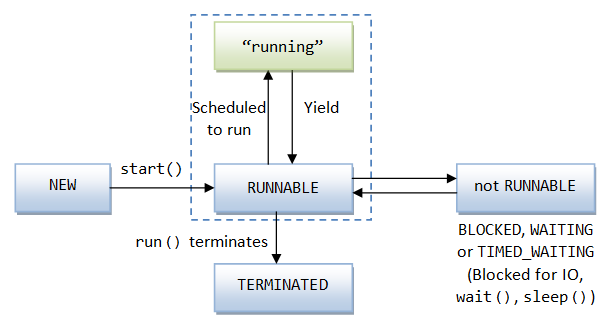
\includegraphics[scale=0.8]{ThreadLifeCycle.png}
\end{figure}
There is a getState() method in Java returning one of the states \textit{new}, \textit{runnable}, \textit{blocked}, \textit{waiting}, \textit{timed waiting} and \textit{terminated}:
\begin{minted}[]{java}
Thread T = new Thread() {
    public void run() {
        System.out.println(Thread.currentThread().getState());
    }
};
T.start();

> RUNNABLE // prints the state to the console
\end{minted}
We notice that Java differentiates some states we simply put into a \textit{not runnable} state. Later in the script we are going to introduce additional concepts related to these states and mention the state diagram again.

\subsection{Summary}
What is important to remember from this section is that threads are primarly a unit of organization for the OS and are what ultimately runs on the CPU. Their lightweight nature is what enables the scheduler to quickly swap them in and out of the CPU and thus creating the illusion of many programs running at the same time. Although Java threads are created by the JVM rather than the OS, they are 1-to-1 mapped to OS threads and hence we can think about them the same way.

% TODO:
% - Add Java methods for controlling threads: Sleep, interrupt, join... also then explain how they relate to the state model
% - Maybe first give some more intuition on how to use threads with examples.
% - find a diagram for SMT to add a digression section`'
% - incorporate last slide of L03-05: Summary of thread states


% \subsection{Bad Interleavings and Data Races}
% A \textit{race condition} is a mistake in your program such that whether the program behaves correctly or not depends on the order in which the threads execute. Race conditions are very common bugs in concurrent programming that, by definition, do not exist in sequential programming. We distinguish two types of race conditions.\\[3mm]
% One kind of race condition is a \textit{bad interleaving}. The key point is that ''what is a bad interleaving'' depends entirely on what you are trying to do. Whether or not it is okay to interleave two bank-account withdraw operations depends on some specification of how a bank is supposed to behave.
% \begin{example}
%     Suppose we have the following implementation of a \texttt{peek} operation on a concurrent stack.
%     \begin{figure}[H]
%         \centering
%         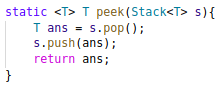
\includegraphics[scale=0.45]{peekWrong.png}
%     \end{figure}
%     \noindent Assume that the \texttt{pop} and \texttt{push} methods are implemented correctly. While \texttt{peek} might look like it's implemented correctly, the following interleaving might occur:
%     \begin{figure}[H]
%         \centering
%         \begin{subfigure}{.5\textwidth}
%             \centering
%             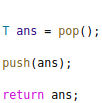
\includegraphics[scale=0.45]{BadInterleaving_1.png}
%             \captionsetup{labelformat=empty}
%             \caption{Thread 1 (\texttt{peek)}}
%         \end{subfigure}%
%         \begin{subfigure}{.5\textwidth}
%             \centering
%             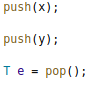
\includegraphics[scale=0.45]{BadInterleaving_2.png}
%             \captionsetup{labelformat=empty}
%             \caption{Thread 2}
%         \end{subfigure}
%     \end{figure}
% \end{example}
% A \textit{data race} is a specific kind of race condition that is better described as a ''simultaneous access error'', although nobody uses that term. There are two kinds of data races:
% \begin{itemize}
%     \item When one thread might read an object field at the same moment that another thread writes the same field.
%     \item When one thread might write an object field at the same moment that another thread also writes the same field.
% \end{itemize}
% \noindent Notice it is not an error for two threads to both read the same object field at the same time.\\[3mm]
% Our programs must never have data races even if it looks like a data race would not cause an error - if our program has data races, the execution of your program is allowed to do very strange things: The exact behavior that the program is allowed to exhibit is usually defined in the memory model of a language, we'll get to the memory model of Java later.
% \begin{example}
%     Let's consider a very simple example.
%     \begin{figure}[H]
%         \centering
%         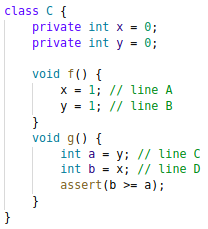
\includegraphics[scale=0.45]{DataRace.png}
%     \end{figure}
%     Notice that \texttt{f} and \texttt{g} are not synchronized, leading to potential data races on fields \texttt{x} and \texttt{y}, Therefore, the assertion in \texttt{g} can fail. But there is no interleaving of operations that justifies the assertion failure, as can be seen through a proof by contradiction: \\[3mm]
%     \quad Assume the assertion fails, meaning \texttt{!(b$>=$a)}. Then \texttt{a==1} and \texttt{b==0}. Since \texttt{a==1}, line B happened before line C. Since A must happen before B, C must happen before D, and ''happens before'' is a transitive relation, A must happen before D. But then \texttt{b==1} and the assertion holds.\\[3mm]
%     There is nothing wrong with the proof except its assumption that we can reason in terms of ''all possible interleavings'' or that everything happens in certain orders. We can reason this way only if the program has no data races.
% \end{example}
%
% \subsection{Other Models}
% We've introduced a programming model of explicit threads with shared memory. This is, of course, not the only programming model for concurrent or parallel programming. Shared memory is often considered convenient because communication uses ''regular'' reads and writes of object fields. However, it's also considered error-prone because communication is implicit; it requires a deep understanding of the code/documentation to know which memory accesses are doing inter-thread communication and which are not. The definition of shared-memory programs is also much more subtle than many programmers think because of issues regarding data races, as discussed in the previous section.\\[3mm]
% Three well-known, popular alternatives to shared memory are presented in the following. Note that different models are better suited for different problems. Models can be abstracted and freely built on top of each other or we can use multiple models in the same program (e.g. MPI with Java).\\[3mm]
% \textit{Message-passing} is the natural alternative to shared memory. In this model, explicit threads do not share objects. For them to communicate, copies of data are exchanged as messages between processes. As objects are not shared between individual threads, the issue of threads wrongly updating fields does not occur. One does, however, have to keep track of the different data copies being passed around through messages. Message passing is especially fitting for processes which are far apart form each other, similar to sending an email, where a copy of the message is sent to the recipient.\\[3mm]
% \textit{Dataflow} provides more structure than having ''a bunch of threads that communicate with each other however they want.'' Instead, the programmer uses primitives to create a directed acyclic graph. A node in the graph performs some computation using inputs that arrive on its incoming edges. This data is provided by other nodes along their outgoing edges. A node starts its computation when all of its inputs are available, something the implementation keeps track of automatically.\\[3mm]
% \textit{Data parallelism} does not have explicit threads or nodes running different parts of the program at different times. Instead, it has primitives for parallelism that involve applying the same operation to different pieces of data at the same time. For example, you would have a primitive for applying some function to every element of an array. The implementation of this primitive would use parallelism rather than a sequential for-loop. Hence all the parallelism is done for you provided you can express your program using the available primitives.
%
\end{document}
